\documentclass{article}
\usepackage[utf8]{inputenc}
\usepackage[T1]{fontenc}
\usepackage{graphicx}
\graphicspath{ {./images/} }

\title{Rapport SYSG5 - Acces Control List}
\author{AZDAD Yassin & BOUAYAD Amer }
\date{03 December 2019}

\begin{document}


\maketitle
\newpage

\tableofcontents

\newpage

\section{Introduction}
En Linux, chaque fichier et dossier possède des permissions. Il existe un schéma traditionnel UNIX (et Linux) qui les décrit. Pour de nombreuses applications, ce schéma est suffisant. Cependant, certaines applications nécessitent un contrôle plus précis des autorisations accordées à des utilisateurs et à des groupes spécifiques. C'est dans ce contexte qu'interviennent les ACL, autrement dit, les Access Control List.\\\\
La mise en place des ACL permet une gestion fine des accès des utilisateurs, des groupes, aux répertoires et aux fichiers d'une partition qui dispose d'un “file system” qui accepte les ACL.

Afin de démontrer l'utilisation et l'intérêt des ACL, nous avons créé plusieurs scripts à ce propos. Nous avons travaillé sous la distribution Linux-Opensuse, sur une partition formatée en ext4.

\subsection{Prérequis}
Afin de pouvoir utiliser et attribuer des ACL, il faut, préalablement,vérifier que le paquet des ACL est installé, et dans le cas échéant où il ne le serait pas, l'installer. Pour ce faire on peut faire usage de la commande :\\\\
\texttt{if grep "CONFIG\_FS\_POSIX\_ACL=y" /boot/config-*; then echo "OK"; else echo apt-get install acl; fi}

\section{Qu'est ce qu'une ACL ?}
\subsection{Définition}
Une ACL est une Access Control List. C'est-à-dire que c'est une liste de permissions accordées sur un fichier ou un dossier à certains utilisateurs. 
Il existe 3 types de permissions :
\begin{itemize}
\item Le droit de lecture - R
\item Le droit d'écriture - W
\item Le droit d'exécution - X
\end{itemize}
Il existe également 3 types d'utilisateurs auxquels on peut accorder ou révoquer des permissions.
\begin{itemize}
\item On peut accorder une/des permission(s) à un utilisateur grâce à son nom.
\item On peut accorder une/des permission(s) à un groupe incluant tous ses utilisateurs grâce à son nom.
\item On peut accorder une/des permission(s) à tous les autres utilisateurs qui ne correspondent à aucune ACL.
\end{itemize}
\newpage
\subsection{Illustrations}
\subsubsection{Visualisation ACL}

Afin de visualiser les ACL attribués à un fichier ou un dossier, il suffit d'utiliser la commande : \\\\
\texttt{getfacl  nom\_de\_fichier}\\\\
Cette commande va nous permettre de visualiser les ACL attribuées à nom\_de\_fichier comme on peut le voir dans l'image ci-dessous. \\
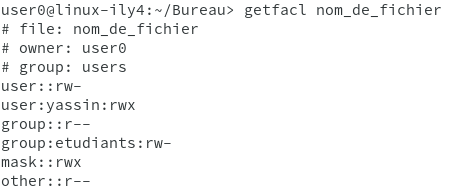
\includegraphics[width=7.5cm]{images/getfacl.png}\\
On peut y voir que l'utilisateur yassin dispose de tous les droits (RWX) sur ce fichier, et que les utilisateurs du groupe étudiants ont seulement le droit de lecture et écriture(RW-) et, pour finir, que les autres utilisateurs (ceux qui n'ont pas déjà été nominés par une ACL) n'ont aucun droit dessus.



\subsubsection{Suppression d'ACL}
Il est aussi possible de supprimer des ACL attribuées à un fichier ou un dossier avec l'option -b. Par exemple via la commande : \\
\texttt{setfacl -b  nom\_de\_fichier} \\\\
Il est également possible de supprimer une seule ou plusieurs parties des ACL attribuées à un fichier. Pour ce faire, il faut utiliser l'option -x. Par exemple via la commande : \\
\texttt{setfacl -x u:michel,g:esi fichier2} \\\\
Cette commande supprimera les permissions de l'utilisateur michel et du groupe esi attribuées au fichier fichier2.

\subsubsection{Autres options possibles}
Il est également possible de copier les ACL d'un fichier file1 à un autre fichier file 2 via la commande :\\
\texttt{getfacl file1 | setfacl --set-file=- file2}\\\\
Il est également possible de supprimer les ACL par défaut d'un fichier file1 avec l'option -k. Par exemple, via la commande :\\
\texttt{setfacl -k file1}
\newpage

\subsubsection{Attribution et vérification d'ACL}
Afin d'illuster et de démontrer l'attribution et la vérification d'ACL, nous avons mis au point un script automatique qui permet de poser des ACL sur des fichiers et de prouver que seuls les utilisateurs autorisés ont la ou les permissions qui leurs ont été attribuées. \newline
\begin{center}
    \textbf{\textit{scriptACL.sh}}
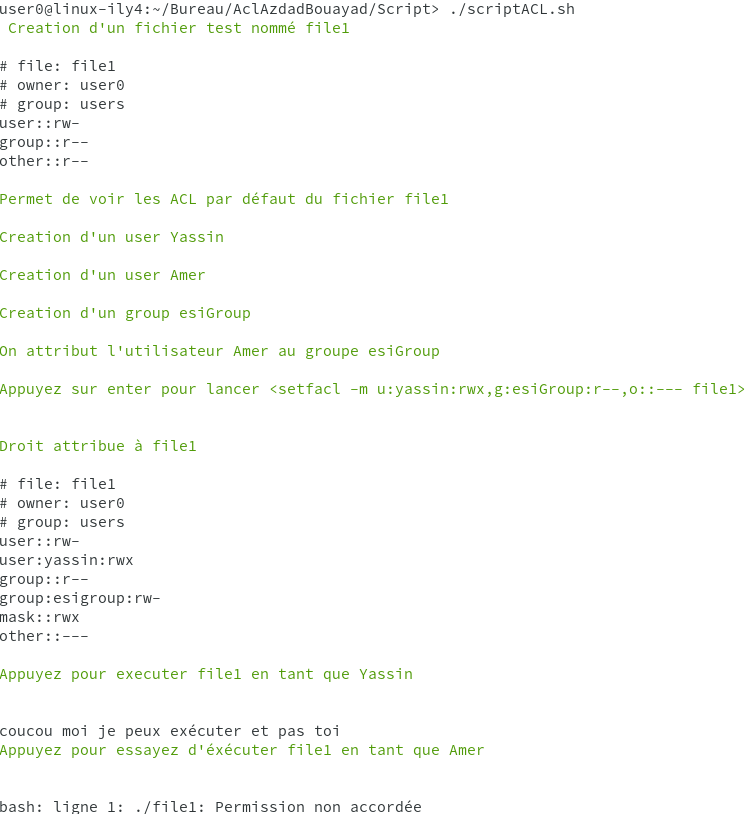
\includegraphics[width=12cm]{images/scriptACL.png}
\end{center}

\newpage

Via ce script et ses sorties, on peut voir et démontrer plusieurs choses : 
\begin{itemize}
\item Qu'on peut attribuer des ACL à un fichier.
\begin{center}
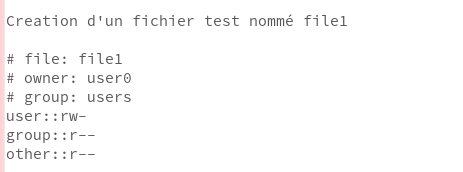
\includegraphics[width=12cm]{images/aclBefore.png}
\end{center}
\begin{center}
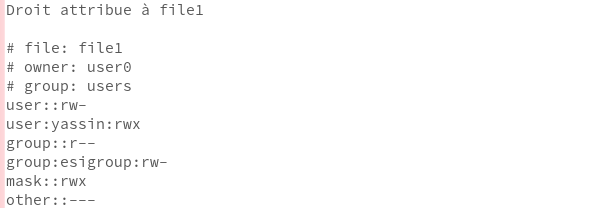
\includegraphics[width=12cm]{images/aclAfter.png}
\end{center}
\item Que l'utilisateur Yassin peut exécuter le fichier file1.
\begin{center}
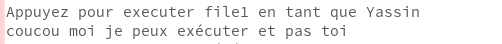
\includegraphics[width=12cm]{images/testYassin.png}
\end{center}
\item Que l'utilisateur Amer ne peut pas exécuter le fichier file1.
\begin{center}
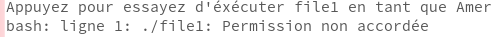
\includegraphics[width=12cm]{images/testAmer.png}
\end{center}
\end{itemize}
\newpage
Voici la sortie totale de l'exécution du script scriptACL.sh

\begin{center}
    \textbf{\textit{sortie du script scriptACL.sh}}
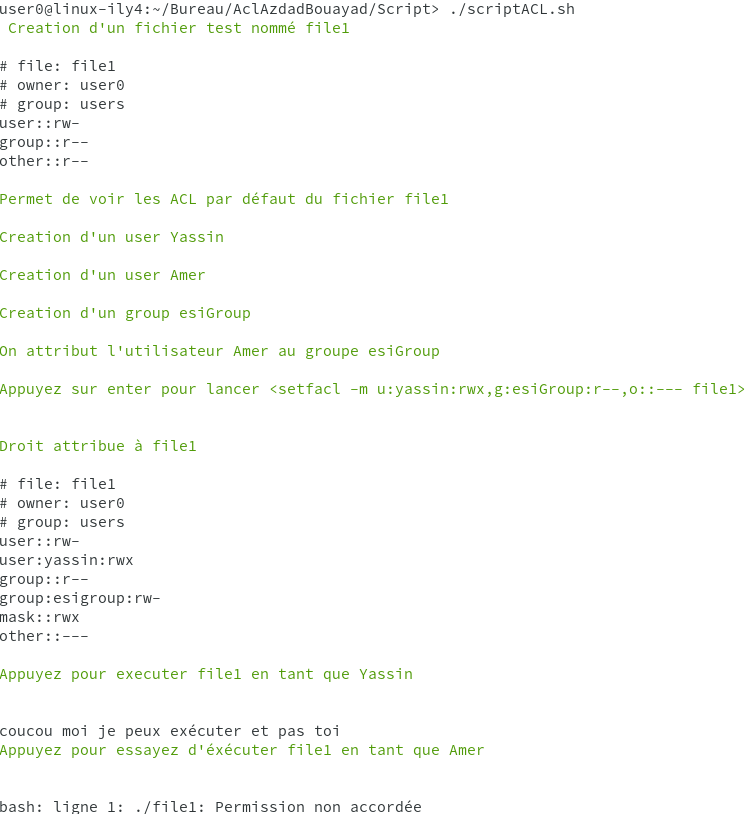
\includegraphics[width=12cm]{images/scriptACL.png}
\end{center}
\newpage
\section{Héritage d'ACL}
Les fichiers incluent dans un dossier n'héritent pas automatiquement des ACL attribués à ce dossier. Pour que ces fichiers puissent en hériter, il faut attribuer des droits par défaut à ce dossier codé \textit{-d}\\\\
Par conséquent, et suite à cela, les fichiers héritent de cet attribut d'ACL par défaut.\\\\
Afin de prouver ce concept, nous avons élaboré un script heritage.sh, qui a permis de démontrer que les fichiers créés dans un dossier à qui des ACL par défaut ont été attribuées, héritent eux-mêmes de ces ACL par défaut.

\begin{center}
    \textbf{\textit{heritageACL.sh}}
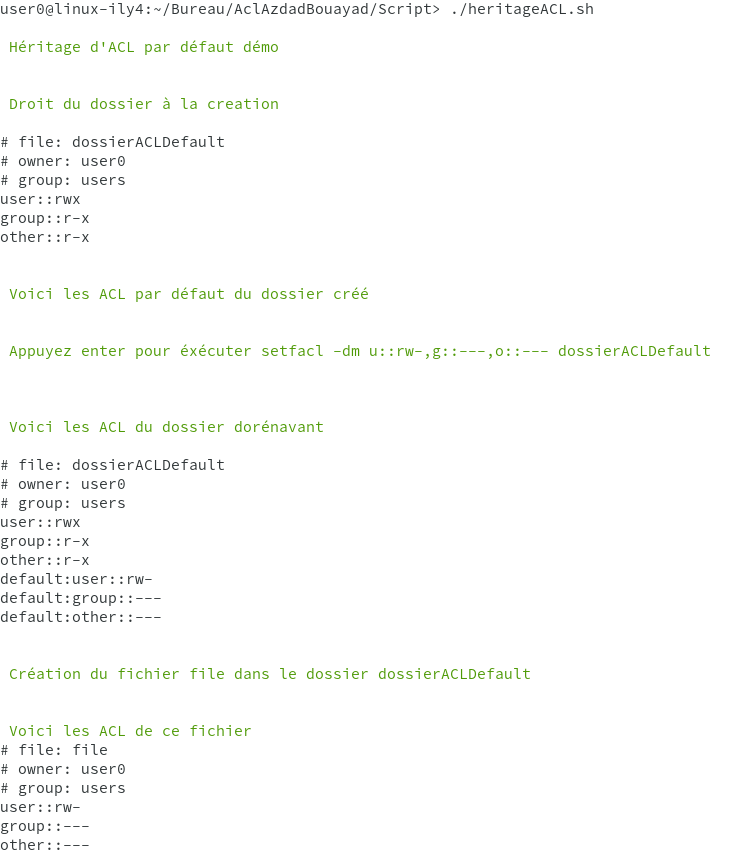
\includegraphics[width=10cm]{images/heritageACL.png}
\end{center}
Ce script a pour but de créer un dossier dossierACLDefault et de lui attribuer des ACL par défaut pour tous les fichiers qui seront créés dedans. De plus, ce script permet de vérifier que cette opération s'est passé sans encombre.

\newpage

\begin{center}
    \textbf{\textit{Sortie script heritageACL.sh}}
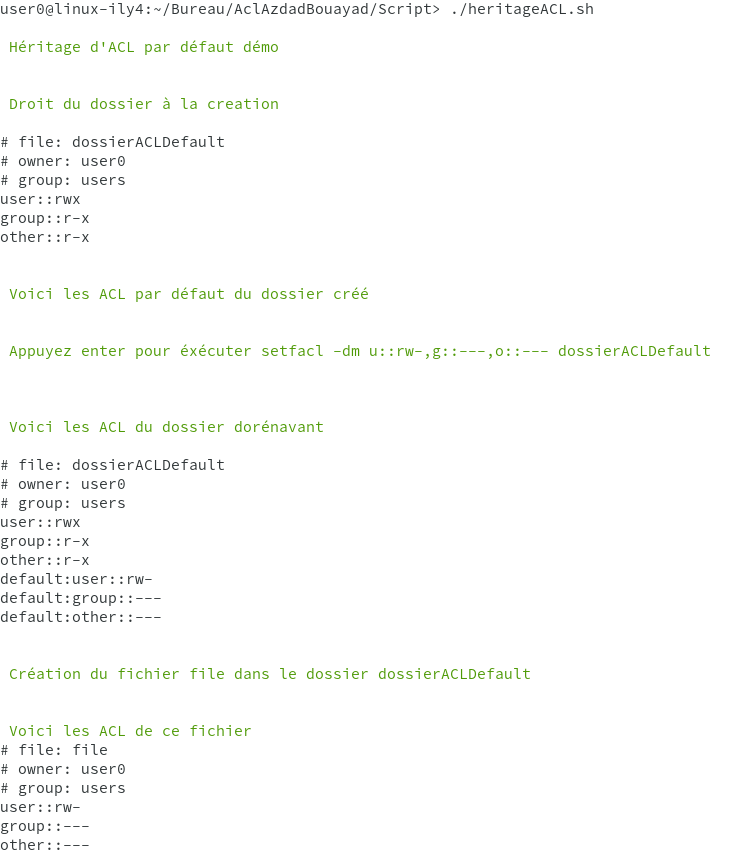
\includegraphics[width=12cm]{images/sortieHeritageACL.png}
\end{center}
On peut facilement se rendre compte que le fichier file créé dans le dossier dossierACLDefault a hérité des ACL par défaut du dossier dossierACLDefault créé préalablement. \\\\
En effet, par défaut, les fichiers créés dans ce dossier étaient censés se voir attribuer le droit de lecture et d'écriture aux users et c'est bien ce qui s'est passé comme on peut le voir après la commande getfacl file.
\newpage
\section{Masque}
Le masque est une des notions propres aux ACL étendues. Avant cela, il faut, bien entendu, faire une différence entre les ACL minimales et les ACL étendues. 

\subsection{ACL minimales}
Les ACL minimales sont des ACL qui contiennent sémantiquement et exclusivement les 3 champs d'attribution : 
\begin{itemize}
\item \texttt{ACL\_USER\_OBJ}: Attribution à un utilisateur.
\item \texttt{ACL\_GROUP\_OBJ}: : Attribution à un groupe.
\item \texttt{ACL\_OTHER}: Attribution aux autres (ni utilisateur, ni dans le groupe)
\end{itemize}
Pour illuster une ACL minimale voici un exemple :\\\\
\texttt{setfacl −m u:yassin:rwx,g:amer:r--,o:-- file1}\\\\
On peut voir que le champ \texttt{ACL\_USER\_OBJ}= yassin, que le champ \texttt{ACL\_GROUP\_OBJ}=amer et que le champ \texttt{ACL\_OTHER} n'a pas, et ne devrait, logiquement, jamais avoir d'assignation d'utilisateur étant donné qu'il s'agit de tous les utilisateurs qui ne se sont pas vu attribué des ACL et que par conséquent il n'y a pas de nom précis pour ces utilisateurs.

\subsection{ACL étendues}
Il existe des ACL étendues qui contiennent un autre champ qui est le masque. Le masque existe lorsqu'une ACL est attribuée à un dossier ou un fichier. 
Le masque est une synthèse des valeurs les plus permissives que possède un fichier doté d'une ACL
L'intérêt du masque est de pouvoir préalablement assigner les permissions qui peuvent être accordées ou non, indépendamment de l'utilisateur. Autrement dit, seuls les droits du masque peuvent être accordés de manière effective.
\newpage
\subsection{Illustration}
Afin de démontrer et d'illustrer ce concept, nous avons élaboré un script scriptMasque.sh que voici :
\begin{center}
    \textbf{\textit{scriptMasque.sh}}
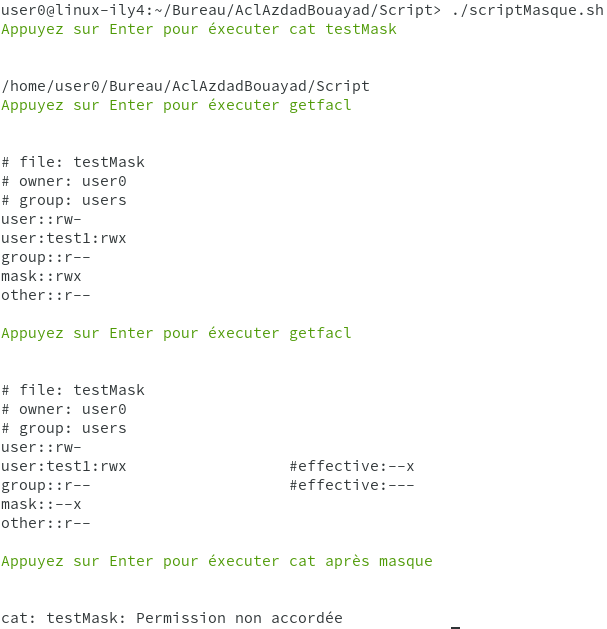
\includegraphics[width=12cm]{images/scriptMasque.png}
\end{center}
Dans ce script, on attribue une ACL, de façon "normale" au fichier testMask, ensuite on visualise ses ACL afin de se rendre compte du masque par défaut attribuer à ce fichier. Puis on modifie ce masque de façon à ce que les droits les plus permissifs soient ceux d'exécution uniquement. Ensuite on essaie de lire le fichier afin de voir si notre masque à réussi à contrer les droits accordés à l'user test1
\newpage
\begin{center}
    \textbf{\textit{sortie scriptMasque.sh}}
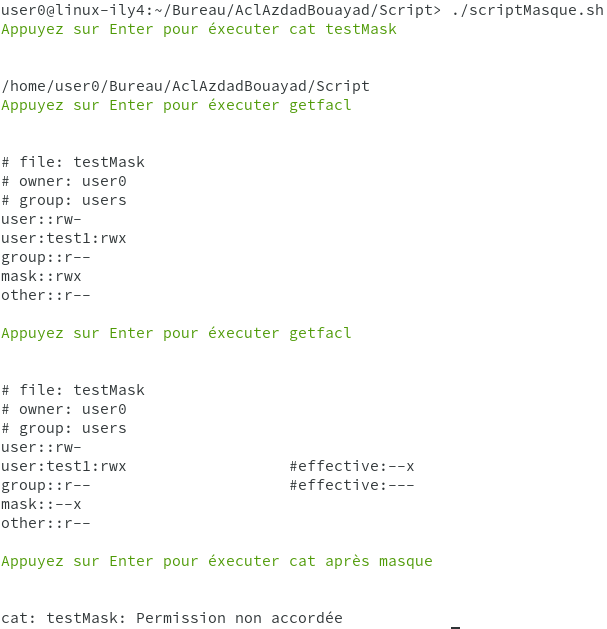
\includegraphics[width=12cm]{images/sortieScriptMasque.png}
\end{center}
On peut se rendre compte grâce à la sortie générée à l'automatisation du script scriptMasque.sh qu'effectivement, malgré le fait que l'user test1 avait tous les droit (RWX), il n'a pas pu lire le fichier testMask car le masque a fait en sorte que les droits permissifs soient seulement ceux d'exécution et que donc seul ce droit pourra être effectué.
\newpage
\section{Localisation d'ACL}
Les ACL sont stockés en tant qu'attributs étendus. Elles sont directement stockés dans les inodes en tant que méta-données. Et dans le cas échéant où la taille de la liste de ces ACL est trop conséquente, un seul bloc supplémentaire peut être utilisé pour le stockage de ces ACL.\\\\
Si le stockage des ACL nécessite un bloc de disque supplémentaire, le champ i\_file\_acl désigne le n° de ce bloc supplémentaire.\\\\
Afin de prouver et démonter tout cela, nous avons élaboré un script scriptLocalisation.sh qui permet d'utiliser le debugger pour voir les stats d'un fichier créé avant et après une attribution d'ACL pour voir le stockage de cette ACL en tant que méta donnée dans l'inode.
\begin{center}
    \textbf{\textit{scriptLocalisation.sh}}
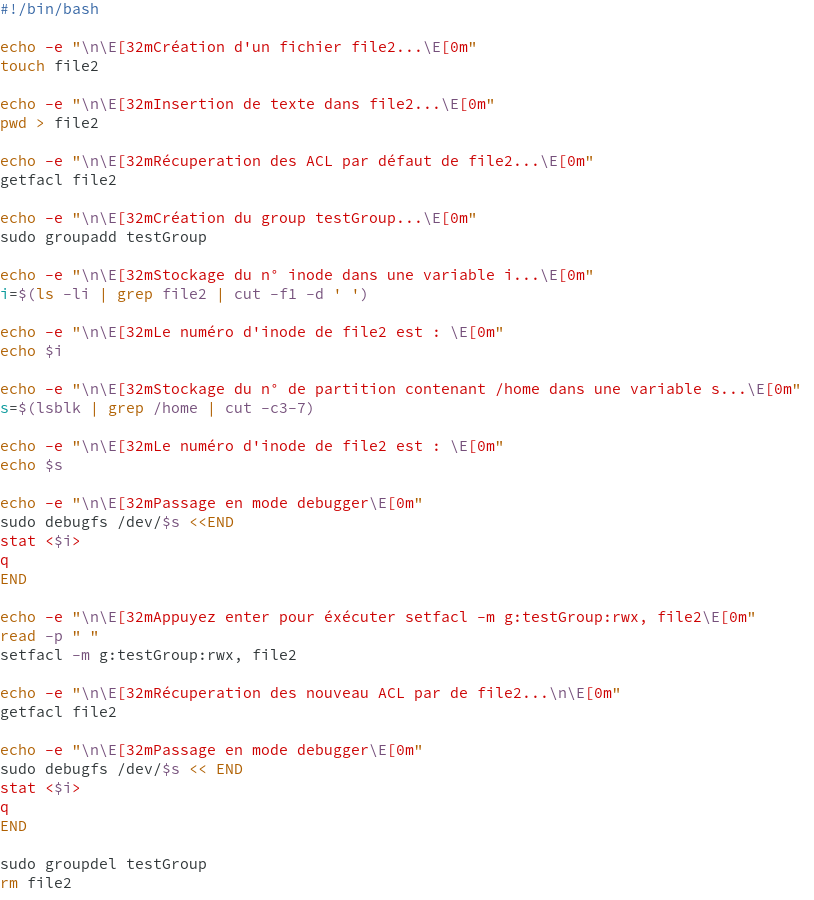
\includegraphics[width=10cm]{images/scriptLocalisation.png}
\end{center}

\newpage
Voici le résultat de la commande stat <n° inode du fichier> avant de poser une ACL dessus. On peut se rendre compte qu'il n'y a pas d'attribut étendus.
\begin{center}
    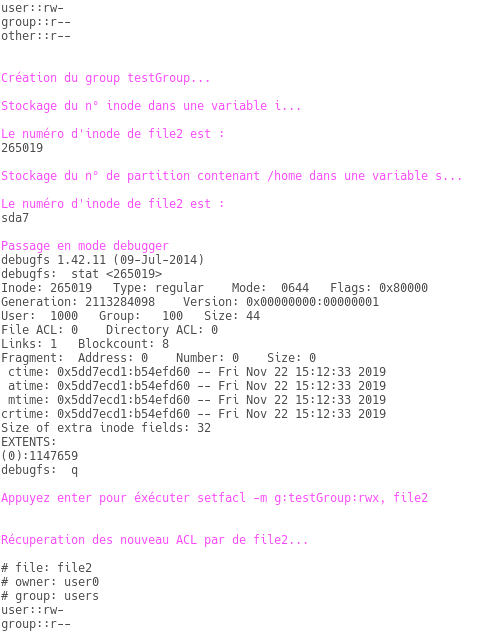
\includegraphics[width=12cm]{images/sortie1Debug.png}
\end{center}
\newpage
Et voici le résultat de la commande stat <n° inode du fichier> après avoir attribuer une ACL au fichier. On peut se rendre compte que désormais il y'a des attributs étendus du fichier. On peut en conclure que les ACL sont bel et bien stockés dans les inodes.  
\begin{center}
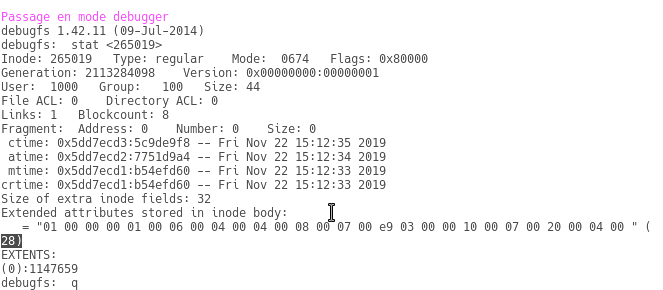
\includegraphics[width=12cm]{images/sortie2Debug.png}
\end{center}

\newpage

\section{Limite d'attribution d'ACL}
Comme précedemment expliqué, les ACL peuvent se voir attribuer une bloc supplémentaire pour leur stockage. Afin de démontrer cela, nous avons élaboré un script qui va attribuer, en boucle, une quantité conséquente d'ACL (508). Voyons comment le système va réagir.
\begin{center}
    \textbf{\textit{scriptLimite.sh}}
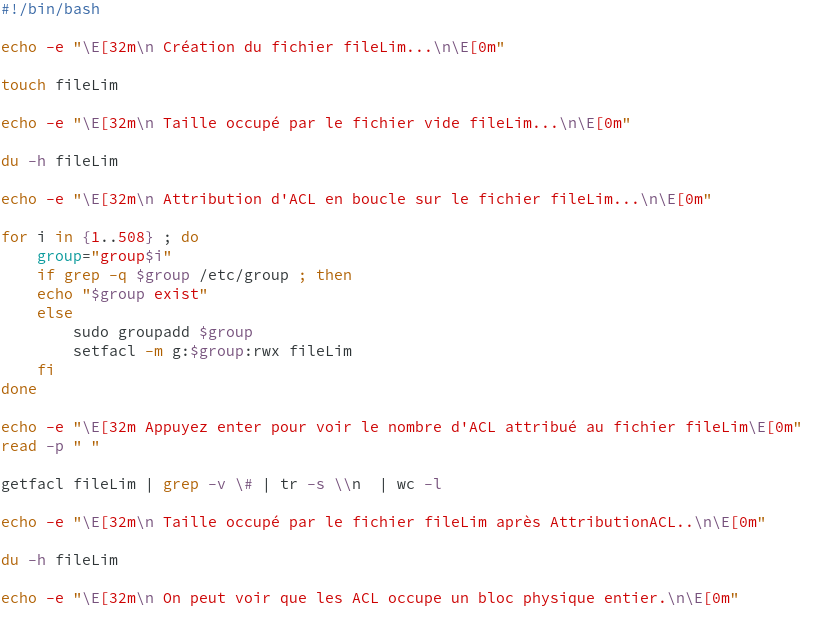
\includegraphics[width=12cm]{images/scriptLimiteAcl.png}
\end{center}
\newpage
\begin{center}
    \textbf{\textit{sortie scriptLimite.sh}}
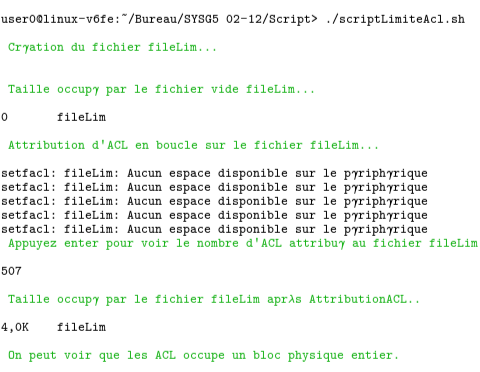
\includegraphics[width=12cm]{images/sortieScriptLimite.png}
\end{center}
Comme nous pouvons le constater, le système ne permet d'attribuer des ACL au fichier fileLim, ce qui démontre le fait qu'il y'a une limite et que justement, seul un bloc est attribué pour le stockage de ces ACL.


\section{Conclusion}
Nous connaissons dans le cadre de nos études, le système d'autorisations par défaut fournit par les systèmes UNIX et Linux.
Celui-ci est pleinement suffisant dans la plupart des utilisations, cependant il ne supervise que 3 catégories d'utilisateur:
le propriétaire, le groupe auquel appartient le propriétaire et les "autres membres".
Alors que ACL permet de superviser plusieurs utilisateurs et groupes spécifiques. 
Les ACL permettent donc d'autoriser un utilisateur tiers sans autoriser tout un groupe ou les "autres membres".
De plus, les ACL sont accès simple d'utilisation à condition que votre noyau le supporte, dans le cas contraire les droits accordés par les ACL
ne seront pas pris en compte.
\newpage
\section{Bibliographie}
\begin{itemize}
\item https://doc.ubuntu-fr.org/acl
\item https://www.geeksforgeeks.org/access-control-listsacl-linux/
\item http://sdz.tdct.org/sdz/les-acl-access-control-lists-sous-linux.html
\item https://lea-linux.org/documentations/Gestion\_des\_ACL
\item https://access.redhat.com/documentation/fr-fr/red\_hat\_enterprise\_linux/6/html/storage\_administration\_guide/acls-setting

\end{itemize}



\end{document}
